% This file was created with tikzplotlib v0.10.1.
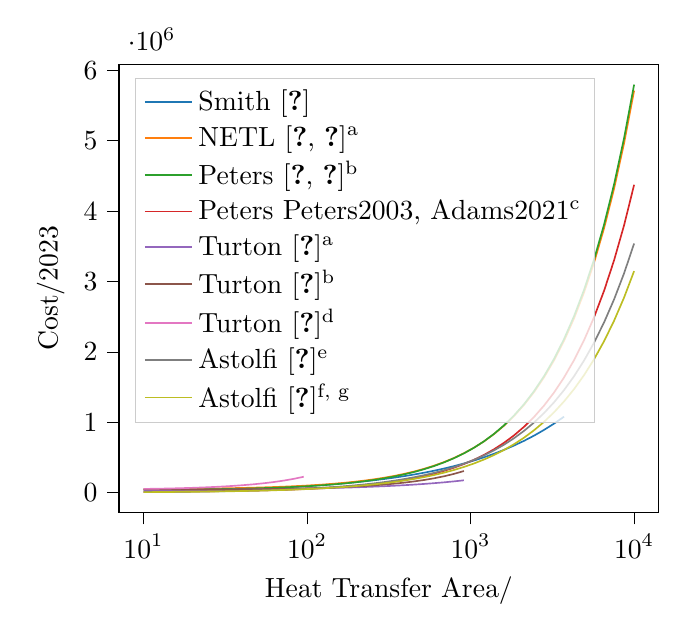
\begin{tikzpicture}

\definecolor{crimson2143940}{RGB}{214,39,40}
\definecolor{darkgray176}{RGB}{176,176,176}
\definecolor{darkorange25512714}{RGB}{255,127,14}
\definecolor{forestgreen4416044}{RGB}{44,160,44}
\definecolor{goldenrod18818934}{RGB}{188,189,34}
\definecolor{gray127}{RGB}{127,127,127}
\definecolor{lightgray204}{RGB}{204,204,204}
\definecolor{mediumpurple148103189}{RGB}{148,103,189}
\definecolor{orchid227119194}{RGB}{227,119,194}
\definecolor{sienna1408675}{RGB}{140,86,75}
\definecolor{steelblue31119180}{RGB}{31,119,180}

\begin{axis}[
legend cell align={left},
legend style={
  fill opacity=0.8,
  draw opacity=1,
  text opacity=1,
  at={(0.03,0.97)},
  anchor=north west,
  draw=lightgray204
},
log basis x={10},
tick align=outside,
tick pos=left,
unbounded coords=jump,
x grid style={darkgray176},
xlabel={Heat Transfer Area/\unit{\square\m}},
xmin=7.07945784384138, xmax=14125.3754462276,
xmode=log,
xtick style={color=black},
xtick={0.1,1,10,100,1000,10000,100000,1000000},
xticklabels={
  \(\displaystyle {10^{-1}}\),
  \(\displaystyle {10^{0}}\),
  \(\displaystyle {10^{1}}\),
  \(\displaystyle {10^{2}}\),
  \(\displaystyle {10^{3}}\),
  \(\displaystyle {10^{4}}\),
  \(\displaystyle {10^{5}}\),
  \(\displaystyle {10^{6}}\)
},
y grid style={darkgray176},
ylabel={Cost/\unit{\USD}2023},
ymin=-283325.074453396, ymax=6088024.18060106,
ytick style={color=black},
ytick={-1000000,0,1000000,2000000,3000000,4000000,5000000,6000000,7000000},
yticklabels={\ensuremath{-}1,0,1,2,3,4,5,6,7}
]
\addplot [semithick, steelblue31119180]
table {%
10 nan
11.5139539932645 nan
13.2571136559011 nan
15.2641796717523 nan
17.5751062485479 nan
20.2358964772516 nan
23.2995181051537 nan
26.8269579527973 nan
30.8884359647748 nan
35.5648030622313 nan
40.9491506238043 nan
47.1486636345739 nan
54.2867543932386 nan
62.5055192527397 nan
71.9685673001152 nan
82.8642772854684 81048.665100301
95.4095476349994 89202.806695768
109.854114198756 98177.3199170556
126.48552168553 108054.74068736
145.634847750124 118925.908701488
167.683293681101 130890.802851458
193.069772888325 144059.460702569
222.29964825262 158552.99047609
255.954792269954 174504.684845477
294.705170255181 192061.246789358
339.322177189533 211384.138775108
390.693993705462 232651.067681031
449.843266896944 256057.619113556
517.947467923121 281819.056149764
596.362331659464 310172.299047746
686.6488450043 341378.104131603
790.60432109077 375723.46188964
910.298177991522 413524.236340344
1048.11313415469 455128.069939622
1206.79264063933 500917.580744846
1389.49549437314 551313.881239092
1599.85871960606 606780.451177123
1842.06996932672 667827.400070563
2120.95088792019 735016.158513022
2442.05309454865 808964.641489938
2811.76869797423 890352.931158519
3237.45754281764 979929.531360644
3727.59372031494 1078518.2513896
4291.93426012878 nan
4941.71336132383 nan
5689.86602901829 nan
6551.28556859551 nan
7543.12006335462 nan
8685.11373751352 nan
10000 nan
};
\addlegendentry{Smith \cite{Smith2005}}
\addplot [semithick, darkorange25512714]
table {%
10 48854.9356223176
11.5139539932645 49713.2847258179
13.2571136559011 50701.5839346041
15.2641796717523 51839.5070967584
17.5751062485479 53149.70659045
20.2358964772516 54658.2642596863
23.2995181051537 56395.2106196636
26.8269579527973 58395.1226674183
30.8884359647748 60697.8121982606
35.5648030622313 63349.1183301495
40.9491506238043 66401.8200126125
47.1486636345739 69916.6866853165
54.2867543932386 73963.6880015136
62.5055192527397 78623.3866980512
71.9685673001152 83988.5423394919
82.8642772854684 90165.9578617171
95.4095476349994 97278.6056737351
109.854114198756 105468.075641522
126.48552168553 114897.393685354
145.634847750124 125754.267099807
167.683293681101 138254.821200279
193.069772888325 152647.901680593
222.29964825262 169220.028327763
255.954792269954 188301.098706369
294.705170255181 210270.95535452
339.322177189533 235566.947223062
390.693993705462 264692.635881902
449.843266896944 298227.819805904
517.947467923121 336840.076291566
596.362331659464 381298.05076677
686.6488450043 432486.758040893
790.60432109077 491425.200093786
910.298177991522 559286.651116956
1048.11313415469 637422.01361665
1206.79264063933 727386.710523503
1389.49549437314 830971.648643851
1599.85871960606 950238.869835134
1842.06996932672 1087562.59960523
2120.95088792019 1245676.51028086
2442.05309454865 1427728.1396023
2811.76869797423 1637341.54804289
3237.45754281764 1878689.46215852
3727.59372031494 2156576.34010829
4291.93426012878 2476534.01291284
4941.71336132383 2844931.8053592
5689.86602901829 3269103.32870396
6551.28556859551 3757492.4692084
7543.12006335462 4319821.47866622
8685.11373751352 4967284.51306375
10000 5712770.47210301
};
\addlegendentry{NETL \cite{Loh2002, Adams2021}\textsuperscript{a}}
\addplot [semithick, forestgreen4416044]
table {%
10 38094.7868383405
11.5139539932645 38967.7461393471
13.2571136559011 39972.8674623254
15.2641796717523 41130.1595293675
17.5751062485479 42462.6602910368
20.2358964772516 43996.8955376218
23.2995181051537 45763.4069420243
26.8269579527973 47797.360045911
30.8884359647748 50139.2442921718
35.5648030622313 52835.6790390717
40.9491506238043 55940.3416012361
47.1486636345739 59515.0357917734
54.2867543932386 63630.9222367569
62.5055192527397 68369.934953661
71.9685673001152 73826.412393254
82.8642772854684 80108.9754137298
95.4095476349994 87342.6895714842
109.854114198756 95671.5547727652
126.48552168553 105261.37184713
145.634847750124 116303.043106936
167.683293681101 129016.372596352
193.069772888325 143654.441680587
222.29964825262 160508.647079197
255.954792269954 179914.50163446
294.705170255181 202258.313289389
339.322177189533 227984.87523229
390.693993705462 257606.320293832
449.843266896944 291712.315859094
517.947467923121 330981.802242385
596.362331659464 376196.508198018
686.6488450043 428256.512617232
790.60432109077 488198.16219443
910.298177991522 557214.701745653
1048.11313415469 636680.027862364
1206.79264063933 728176.038759121
1389.49549437314 833524.124762368
1599.85871960606 954821.426314354
1842.06996932672 1094482.58127202
2120.95088792019 1255287.7925549
2442.05309454865 1440438.17301373
2811.76869797423 1653619.46925756
3237.45754281764 1899075.43297516
3727.59372031494 2181692.30033683
4291.93426012878 2507096.06118913
4941.71336132383 2881764.45435798
5689.86602901829 3313155.91852563
6551.28556859551 3809858.06567696
7543.12006335462 4381758.63274256
8685.11373751352 5040242.31453409
10000 5798417.3962804
};
\addlegendentry{Peters \cite{Peters2003, Adams2021}\textsuperscript{b}}
\addplot [semithick, crimson2143940]
table {%
10 12376.5836909871
11.5139539932645 13037.6951281512
13.2571136559011 13798.8957953439
15.2641796717523 14675.3387415139
17.5751062485479 15684.4711175061
20.2358964772516 16846.3814925349
23.2995181051537 18184.1997527728
26.8269579527973 19724.5575427455
30.8884359647748 21498.1184154368
35.5648030622313 23540.1882446789
40.9491506238043 25891.4180511717
47.1486636345739 28598.6132331267
54.2867543932386 31715.6653107083
62.5055192527397 35304.6247322968
71.9685673001152 39436.9360986831
82.8642772854684 44194.8603945246
95.4095476349994 49673.1125391001
109.854114198756 55980.7468547146
126.48552168553 63243.3279863467
145.634847750124 71605.430488543
167.683293681101 81233.516838268
193.069772888325 92319.2511656591
222.29964825262 105083.314668373
255.954792269954 119779.798662107
294.705170255181 136701.262718768
339.322177189533 156184.558583476
390.693993705462 178617.535805816
449.843266896944 204446.762572813
517.947467923121 234186.415440493
596.362331659464 268428.514929906
686.6488450043 307854.710745294
790.60432109077 353249.851220076
910.298177991522 405517.607114517
1048.11313415469 465698.460784494
1206.79264063933 534990.418827645
1389.49549437314 614772.860528849
1599.85871960606 706633.996850646
1842.06996932672 812402.486588464
2120.95088792019 934183.839066292
2442.05309454865 1074402.32803302
2811.76869797423 1235849.25112981
3237.45754281764 1421738.49561887
3727.59372031494 1635770.51650784
4291.93426012878 1882206.00066794
4941.71336132383 2165950.68336067
5689.86602901829 2492653.00559642
6551.28556859551 2868816.55636793
7543.12006335462 3301929.53812055
8685.11373751352 3800613.83269907
10000 4374796.63519313
};
\addlegendentry{Peters \citea{Peters2003, Adams2021}\textsuperscript{c}}
\addplot [semithick, mediumpurple148103189]
table {%
10 36947.3604759323
11.5139539932645 37123.8539504014
13.2571136559011 37406.5523720989
15.2641796717523 37797.8676069801
17.5751062485479 38301.1581109986
20.2358964772516 38920.7770126433
23.2995181051537 39662.13491567
26.8269579527973 40531.7786915178
30.8884359647748 41537.4878688169
35.5648030622313 42688.3906074866
40.9491506238043 43995.1016777298
47.1486636345739 45469.885361979
54.2867543932386 47126.8467749011
62.5055192527397 48982.1557699135
71.9685673001152 51054.308390545
82.8642772854684 53364.43175559
95.4095476349994 55936.6393674391
109.854114198756 58798.4451382589
126.48552168553 61981.2459811849
145.634847750124 65520.8846646748
167.683293681101 69458.3068399317
193.069772888325 73840.328799578
222.29964825262 78720.5357028886
255.954792269954 84160.333821597
294.705170255181 90230.1849584617
339.322177189533 97011.0567373504
390.693993705462 104596.129165964
449.843266896944 113092.805985344
517.947467923121 122625.089158015
596.362331659464 133336.386796181
686.6488450043 145392.83937149
790.60432109077 158987.266770692
910.298177991522 174343.860401553
1048.11313415469 nan
1206.79264063933 nan
1389.49549437314 nan
1599.85871960606 nan
1842.06996932672 nan
2120.95088792019 nan
2442.05309454865 nan
2811.76869797423 nan
3237.45754281764 nan
3727.59372031494 nan
4291.93426012878 nan
4941.71336132383 nan
5689.86602901829 nan
6551.28556859551 nan
7543.12006335462 nan
8685.11373751352 nan
10000 nan
};
\addlegendentry{Turton \cite{Turton2012}\textsuperscript{a}}
\addplot [semithick, sienna1408675]
table {%
10 47960.468604936
11.5139539932645 46666.6489899994
13.2571136559011 45658.2298004642
15.2641796717523 44918.0378973173
17.5751062485479 44433.6243722527
20.2358964772516 44196.9149783664
23.2995181051537 44203.9854155278
26.8269579527973 44454.9526987188
30.8884359647748 44953.9783916106
35.5648030622313 45709.3838307106
40.9491506238043 46733.881814719
47.1486636345739 48044.9338068759
54.2867543932386 49665.2467263349
62.5055192527397 51623.429147277
71.9685673001152 53954.8334852949
82.8642772854684 56702.6188972692
95.4095476349994 59919.0796096943
109.854114198756 63667.2957968541
126.48552168553 68023.1796898253
145.634847750124 73078.0092578576
167.683293681101 78941.5667952296
193.069772888325 85746.0316737337
222.29964825262 93650.8174861541
255.954792269954 102848.596575743
294.705170255181 113572.823173524
339.322177189533 126107.154889242
390.693993705462 140797.287557736
449.843266896944 158065.869014019
517.947467923121 178431.354744956
596.362331659464 202531.927968172
686.6488450043 231155.949300266
790.60432109077 265280.854885436
910.298177991522 306123.024757088
1048.11313415469 nan
1206.79264063933 nan
1389.49549437314 nan
1599.85871960606 nan
1842.06996932672 nan
2120.95088792019 nan
2442.05309454865 nan
2811.76869797423 nan
3237.45754281764 nan
3727.59372031494 nan
4291.93426012878 nan
4941.71336132383 nan
5689.86602901829 nan
6551.28556859551 nan
7543.12006335462 nan
8685.11373751352 nan
10000 nan
};
\addlegendentry{Turton \cite{Turton2012}\textsuperscript{b}}
\addplot [semithick, orchid227119194]
table {%
10 51866.0790695367
11.5139539932645 54011.5117678878
13.2571136559011 56631.0042674539
15.2641796717523 59784.308165023
17.5751062485479 63545.5535258875
20.2358964772516 68006.1424499846
23.2995181051537 73278.4254803955
26.8269579527973 79500.366737196
30.8884359647748 86841.4666498077
35.5648030622313 95510.2939388424
40.9491506238043 105764.087863507
47.1486636345739 117921.036940429
54.2867543932386 132376.033960443
62.5055192527397 149620.966458045
71.9685673001152 170270.950599716
82.8642772854684 195098.387607057
95.4095476349994 225077.360905348
109.854114198756 nan
126.48552168553 nan
145.634847750124 nan
167.683293681101 nan
193.069772888325 nan
222.29964825262 nan
255.954792269954 nan
294.705170255181 nan
339.322177189533 nan
390.693993705462 nan
449.843266896944 nan
517.947467923121 nan
596.362331659464 nan
686.6488450043 nan
790.60432109077 nan
910.298177991522 nan
1048.11313415469 nan
1206.79264063933 nan
1389.49549437314 nan
1599.85871960606 nan
1842.06996932672 nan
2120.95088792019 nan
2442.05309454865 nan
2811.76869797423 nan
3237.45754281764 nan
3727.59372031494 nan
4291.93426012878 nan
4941.71336132383 nan
5689.86602901829 nan
6551.28556859551 nan
7543.12006335462 nan
8685.11373751352 nan
10000 nan
};
\addlegendentry{Turton \cite{Turton2012}\textsuperscript{d}}
\addplot [semithick, gray127]
table {%
10 7062.58704859496
11.5139539932645 8017.99635516461
13.2571136559011 9102.65106951462
15.2641796717523 10334.03519072
17.5751062485479 11731.9979100038
20.2358964772516 13319.0735680805
23.2995181051537 15120.8448955379
26.8269579527973 17166.3553914782
30.8884359647748 19488.5774877231
35.5648030622313 22124.9440451136
40.9491506238043 25117.9517493145
47.1486636345739 28515.8461325118
54.2867543932386 32373.3992631497
62.5055192527397 36752.7926396124
71.9685673001152 41724.6195195793
82.8642772854684 47369.0228420154
95.4095476349994 53776.987084435
109.854114198756 61051.8048794195
126.48552168553 69310.7420313908
145.634847750124 78686.9277727352
167.683293681101 89331.5007290998
193.069772888325 101416.045185567
222.29964825262 115135.35692489
255.954792269954 130710.583221484
294.705170255181 148392.787606037
339.322177189533 168466.996862662
390.693993705462 191256.795493809
449.843266896944 217129.541713032
517.947467923121 246502.289044353
596.362331659464 279848.508980934
686.6488450043 317705.7230684
790.60432109077 360684.167437505
910.298177991522 409476.629453342
1048.11313415469 464869.615042147
1206.79264063933 527756.026706422
1389.49549437314 599149.556590609
1599.85871960606 680201.026605075
1842.06996932672 772216.939001654
2120.95088792019 876680.536425162
2442.05309454865 995275.710916599
2811.76869797423 1129914.14726715
3237.45754281764 1282766.13825797
3727.59372031494 1456295.56850944
4291.93426012878 1653299.63085892
4941.71336132383 1876953.91547196
5689.86602901829 2130863.59849682
6551.28556859551 2419121.55539371
7543.12006335462 2746374.33569129
8685.11373751352 3117897.06264522
10000 3539678.46513711
};
\addlegendentry{Astolfi \cite{Astolfi2014B}\textsuperscript{e}}
\addplot [semithick, goldenrod18818934]
table {%
10 6281.70986726107
11.5139539932645 7131.48404024569
13.2571136559011 8096.21356142861
15.2641796717523 9191.44930597114
17.5751062485479 10434.8458329612
20.2358964772516 11846.4459665715
23.2995181051537 13449.0038746526
26.8269579527973 15268.3518525994
30.8884359647748 17333.8167248313
35.5648030622313 19678.6925760354
40.9491506238043 22340.7774323215
47.1486636345739 25362.9825432784
54.2867543932386 28794.0240861975
62.5055192527397 32689.2084423346
71.9685673001152 37111.3237034011
82.8642772854684 42131.6517788479
95.4095476349994 47831.1174185204
109.854114198756 54301.592672255
126.48552168553 61647.3778135437
145.634847750124 69986.8825988891
167.683293681101 79454.5349637656
193.069772888325 90202.9479222505
222.29964825262 102405.379599476
255.954792269954 116258.526051186
294.705170255181 131985.691889017
339.322177189533 149840.389820123
390.693993705462 170110.427123614
449.843266896944 193122.544935425
517.947467923121 219247.685124165
596.362331659464 248906.969656899
686.6488450043 282578.488838749
790.60432109077 320805.007848755
910.298177991522 364202.715796839
1048.11313415469 413471.158331571
1206.79264063933 469404.513906524
1389.49549437314 532904.395472065
1599.85871960606 604994.383948337
1842.06996932672 686836.527750531
2120.95088792019 779750.074329103
2442.05309454865 885232.735666439
2811.76869797423 1004984.8305173
3237.45754281764 1140936.69255185
3727.59372031494 1295279.78620444
4291.93426012878 1470502.0317975
4941.71336132383 1669427.90936079
5689.86602901829 1895263.98759614
6551.28556859551 2151650.61188786
7543.12006335462 2442720.58453944
8685.11373751352 2773165.78312747
10000 3148312.79082172
};
\addlegendentry{Astolfi \cite{Astolfi2014B}\textsuperscript{f, g}}
\end{axis}

\end{tikzpicture}
